\documentclass{article}
\usepackage[round]{natbib}
\usepackage{amsmath,amssymb,amsfonts, bbm}%
\usepackage{geometry}%
\usepackage{color}
\usepackage{graphicx}
\usepackage{authblk}
\usepackage{nameref}
\usepackage[right]{lineno}
\usepackage{subcaption}
\usepackage{tikz}

%\usepackage{subcaption}

\newcommand{\noderef}[1]{\textsf{#1}}
\newcommand{\tsinfer}[0]{\texttt{tsinfer}}
\newcommand{\kwarg}[0]{\texttt{KwARG}}
\newcommand{\argweaver}[0]{\texttt{ARGweaver}}
\newcommand{\argweaverD}[0]{\texttt{ARGweaver-D}}
\newcommand{\relate}[0]{\texttt{Relate}}
\newcommand{\espalier}[0]{\texttt{Espalier}}
\newcommand{\arbores}[0]{\texttt{Arbores}}

% Bold the 'Figure #' in the caption and separate it from the title/caption with a period
% Captions will be left justified
\usepackage[aboveskip=1pt,labelfont=bf,labelsep=period,justification=raggedright,singlelinecheck=off]{caption}
\renewcommand{\figurename}{Fig}

% deal with supplementary items
\newcommand{\supplementarysection}{%
  \setcounter{figure}{0}% Reset figure counter
  \let\oldthefigure\thefigure% Capture figure numbering scheme
  \renewcommand{\thefigure}{S\oldthefigure}% Prefix figure number with S
  \section{Supplementary section}% Set supplementary section
}

\begin{document}

\linenumbers
\title{Computing likelihoods under the SMC for a general class of ARGs.}

% First authors
\author[1, $\dagger$]{Gertjan Bisschop}

% Middle Authors
\author[2]{Alison Etheridge}
\author[3]{Peter Ralph}

% last author
\author[1]{Jerome Kelleher}
\affil[$\dagger$]{Denotes corresponding author}

\maketitle

\affil[1]{Big Data Institute, Li Ka Shing Centre for Health Information and Discovery, University of Oxford, OX3 7LF, UK}
\affil[2]{Department of Statistics, University of Oxford, OX1 3LB, UK}
\affil[3]{University of Oregon, USA}

\section{Abstract}
%% WHAT IS THE MAIN FOCUS OF THE PAPER?

\section{Introduction}


% Main motivation:
Major progress in ARG inference. 

Result is whole range of inference methods, all inferring an ARG with their own specific 
characteristics.
Many of these scalable heuristic methods do not explicitly infer recombination events.

%ARGs that are inferred here lack information to enable us to compute 
% a likelihood under the Hudson coalescent.
% Missing: exact time to recombination + non-inferrable recombinations

Currently no way to connect the output of the diverse range of ARG inference methods back 
to a model that would allow us to perform a probabilistic exploration of the 
ARG space around the point estimate, (or likelihood-based inference, ...)


% What are ARGs, their relevance and importance

% associating likelihoods with ARGs

% previous likelihood calculations on ARGs Kuhner and Felsenstein (2000), ARGweaver

% history of approximating the coalescent: 
%SMC (McVean and Cardin, 2005) SMC' (Marjoram and Wall, 2006).
%Also heuristic approximations: Li and Stephens (2003) extending Stephens and Donnelly (2000)
%These have enabled (scalable) ARG inference methods: ARGweaver (relying on SMC, limited 
%to smaller samples, but ability to sample from posterior, and full ARG), and Relate, 
%tsinfer/tsdate (copying algorithm), ArgNeedle (using SMC) 
%Clear distinction into two groups: ARGWeaver infers actual ARG.
% what does kwarg do?
%Whereas the other approaches are heuristic in nature. For example, where ARGweaver has 
%the built in assumption of neighbouring trees being separated by single Subtree Prune 
%Regraft (SPR) (Song citation?), this is not the case for any of the heuristic data 
%structures. (other peculiarities: ...).

% computing likelihoods on ARGs; from Kuhner and Felsenstein to ARGWeaver

% SMC and relatives are useful: lot of focus however on integrating over the distribution of trees to get Ne(t). \cite{PSMC, ...}
% Here the idea is to use the SMC in a different way that resonates more with the true direction of flow
% of genetic/haplotype information.


% results in a concrete way to compute likelihoods for *any* inferred ARG (integrating out the recombination time)
% meaning: e.g. no requirements on adjacent trees only differing by a single SPR, (other?)

% In this paper, we attempt to address these problems by
% providing a precise definition of an ARG that is general enough to encompass
% the output of popular simulation and inference methods.

% ADD: remark on fact that we are only dealing with topology and branch length information
% adding likelihood of observing particular mutation configuration given an ARG is straightforward. 


\section{Methods and Results}
\subsection{SMC backwards-in-time}\label{par:description}

Formulated backwards-in-time, the SMC \citep{mcvean_approximating_2005} only requires a 
simple modification to the 
coalescent with recombination. By only considering those pairs of 
lineages that share 
genomic intervals with ancestral material, as eligible for coalescence, we obtain the 
sequential Markovian structure along the chromosome.\\

More formally, and following the notation of \citet{mcvean_approximating_2005}, at any 
point in time, the process can be described by $L(t)$, the set of labeled lineages 
extant at time $t$ each represented by a union of ordered non-overlapping half open 
intervals detailing the ancestral material 
carried by that lineage $X_i = \{[x_{i0}, y_{i0}), \dotsc, [x_{im}, y_{im})\}$.
$L(0)$ consists of $n$ sampled lineages, labelled $0$ to $n-1$, each represented by a 
single interval spanning the entire genome.
Backwards in time the process evolves by a succession of coalescence and recombination 
events until all segments of ancestral material are each present in only one lineage. 
The waiting time to next event is determined by these two competing processes with exponentially 
distributed waiting times as outlined below.\\

Recombination is described by a Poisson process of rate $r$ per unit of length and time. 
A recombination to the 
left of $x$ with $x>x_{i0}$ and $x<y_{im}$ splits a lineage $i$ into two new, uniquely 
labelled lineages.\\

Any two \emph{overlapping} lineages coalesce at rate $\lambda = 1/(2N_e)$ in the case
of a diploid population of constant size. The newly formed lineage acquires the 
union of both ordered intervals.
Although coalescence is reciprocal, here we'll define a strict total order 
(see \ref{par:liks}) on 
all lineages in $X(t)$ based on their leftmost starting points. 
For any such strict total order on $X(t)$ and at any point in the process 
the instantaneous rate of coalescence then equals $\lambda \sum_{i \neq j} I_{ij}$.

\begin{equation} \label{def:coal}
I_{ij} = \begin{cases}
1 & X_i > X_j \wedge X_i \cap X_j \neq \emptyset \\
0 & \text{otherwise}
\end{cases}
\end{equation}

We can now define $C_i(t) = \{X_j \in L(t) | I_{ij}(t) = 1\}$ such that $|C_i(t)| = 
I_{i}(t) = \sum_{j} I_{ij}(t)$.
Because $I_{ij}$ is not reciprocal, each extant lineage has their own unique set of 
lineages $C_i(t)$ it can coalesce with. This will simplify the likelihood computations 
(see \ref{par:liks). Note that although recombination affects $C_i(t)$ it does not 
affect $I_{i}$.\\ 

% note on the disjoint set of intervals for each lineage under the SMC
As noted by \cite{mcvean_approximating_2005}, the backwards-in-time description of the 
SMC is slightly different from the left-to-right approach in that recombination 
in non-ancestral material is possible (see fig.\ref{fig:smc-unary}). 
Although this does not affect the distribution 
of marginal genealogies, it does mean that not all lineages in $L$ can be represented 
by a single interval. More precisely, all lineages will be associated with 
a single interval up to the point where one section of the 
genome has reached its most recent common ancestor but the neighbouring parts have not.

\subsection{Recording an ARG} \label{par:recording}

The process described in the previous paragraph details the transitions of the 
set of labeled lineages $L$ through time. An Ancestral Recombination Graph 
$\mathcal{G} = (N, E)$ capturing the various inheritance paths along the genome 
is obtained by registering a tuple $(c, p, X_{cp})$ whenever a 
lineage $c$, associated with a disjoint set of genomic intervals $X_c$, is 
replaced by one or two lineage(s), $p$ (and $p^{\prime}$), 
in case of a coalescence or recombination respectively.
The last element of the tuple is the extent of the edge. It is itself a  
disjoint set of intervals such that $X_{cp} \cup X_{cp^{\prime}} = X_c$. 
The set of edges $E$, containing all such tuples $(c, p, X_{cp})$, 
and $N$, the set of nodes representing all genomes in the ARG, together
define this data structure.\\

Recording the full process as described above will result in unary nodes.
These are nodes that have only one child in one or more local trees 
(see fig.\ref{fig:smc-unary} and \citet{Wong-2023}). This is not only true 
for the nodes registered for those lineages affected by a recombination event. 
Coalescence between two lineages without perfectly 
overlapping intervals will similarly result in locally 
unary nodes (see \ref{fig:smc-unary}).These unary nodes ensure the one 
to one correspondence between an ARG and its 
representation as a sequence of local trees. 
Indeed, the presence of these unary nodes allow us to completely reconstruct 
the state of all extant lineages through time from the local trees.\\

%under the SMC up to the exact time of the recombination events.

The resulting data structure can be simplified to various degrees \citep{Wong-2023}. 
This equates to removing certain types of unary nodes, 
depending on the degree of information 
we want to retain (or can reconstruct) from the original process. 
In a fully simplified ARG, without unary nodes, 
the local trees only store information on local coalescence events.
Under the SMC, if we only omit recombination nodes, % is there a better word?
we are left with the coalescent nodes, those nodes that are coalescent 
along some fraction of the genome. We can however still identify \emph{all} 
lineages that were hit by a recombination event and constrain the time to 
this event to within a window defined by the age of the node $c$ associated with that 
lineage and the minimum age of the parents of the edges connecting to $c$.

As highlighted in fig.\ref{fig:smc-unary}, (coalescing) unary nodes can be inferred 
from the available haplotype information. Currently, the following methods 
return the full this information by default as part of their ARG reconstruction algorithm: 
\argweaver \citep{rasmussen_genome-wide_2014} 
\tsinfer \citep{kelleher_inferring_2019}, 
\kwarg \citep{ignatieva_kwarg_2021}.

The presence of these (coalescing) unary nodes enables us to extend likelihood 
computations to a more general class of ARGs.
Here we will compute the likelihood for an ARG
under the SMC for which we have no information on the time to any 
of the recombination events. 
We will assume however, that the identity 
of the lineage involved in each recombination event can be correctly 
inferred by relying on the unary nodes.


\begin{figure}[!ht]
\centering
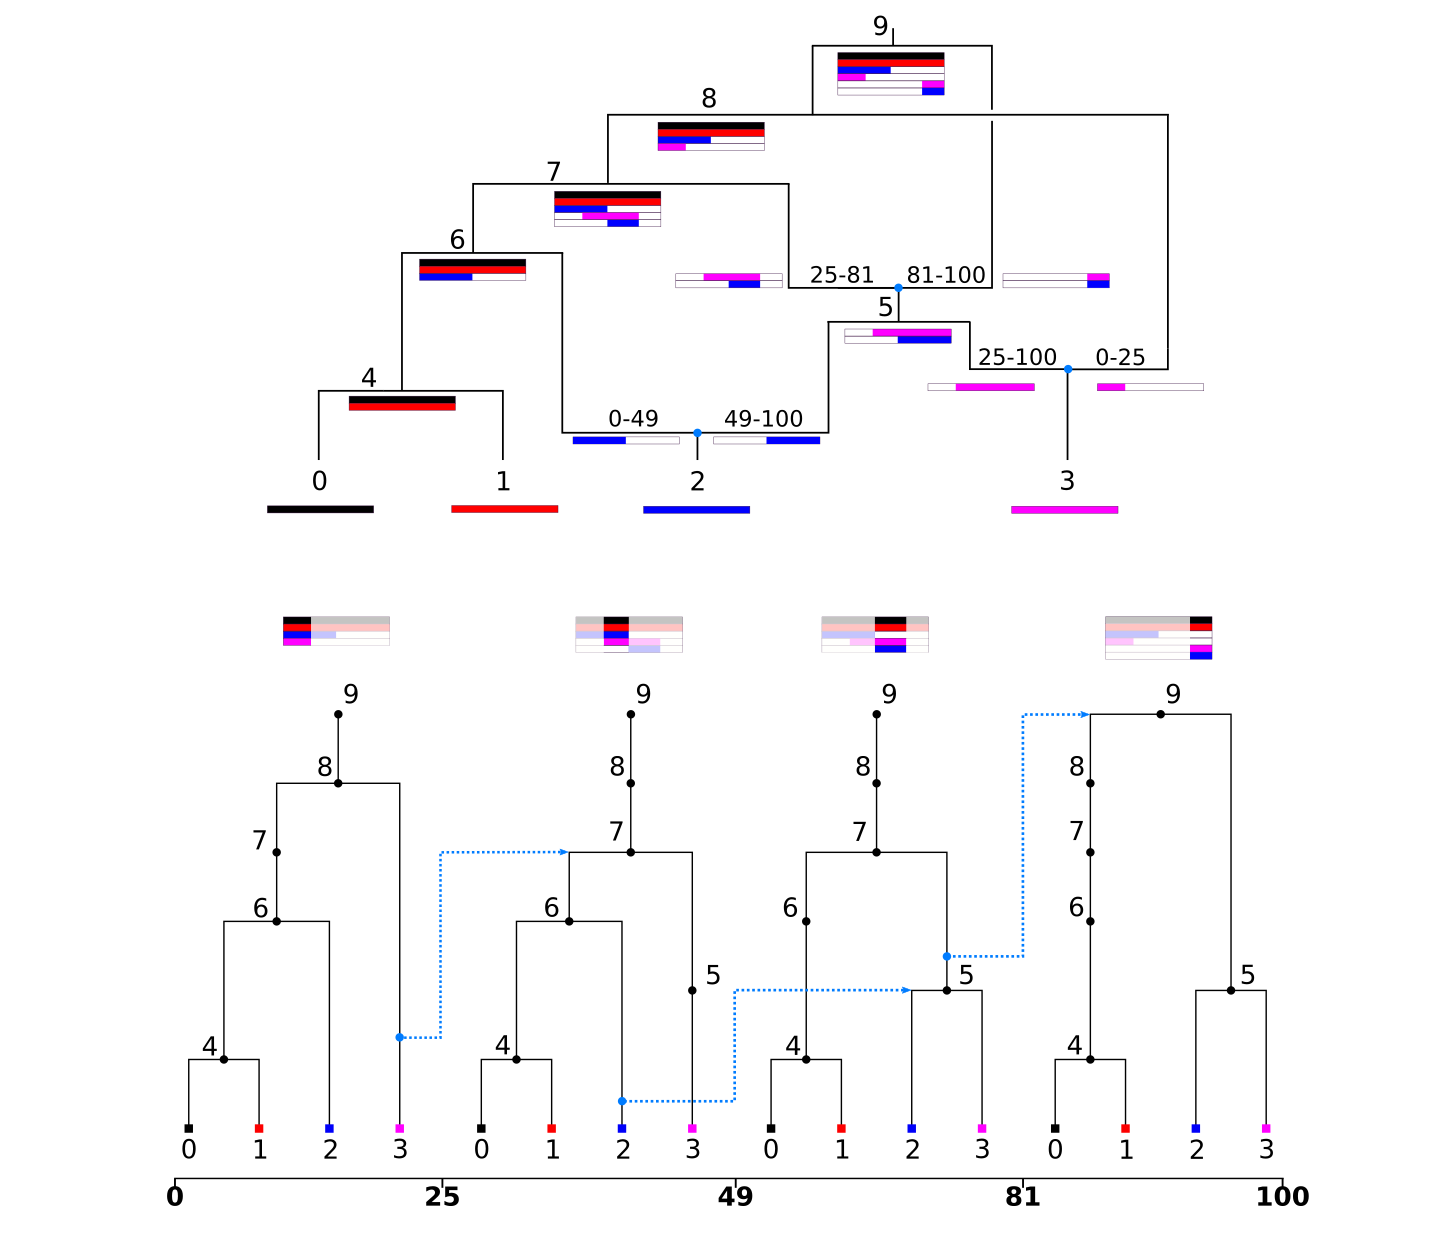
\includegraphics[width=\textwidth]{figures/smc_custom_2rows.png}
\caption{ARG (top left) generated under the SMC and its representation as a 
series of local trees. The presence of the unary nodes in the local trees 
ensure these two representations contain the same information. 
The ARG is augmented with haplotype information, coloured according to the 
samples that inherit from it. 
Note how the presence of a unary node on a local tree is 
indicative of either a past (to the left of the local tree) 
or future (to the right) coalescence event. It therefore modifies the 
left-to-right logic of the SMC whereby the floating lineage coalesces randomly
with a the remaining portion of the local tree. 
}
\label{fig:smc-unary}
\end{figure}

%\subsection{Unary nodes} \label{par:unary}
% Do we need a seperate section on the unary nodes?
% is there more to be said about the SMC inm the presence of unary nodes?
%Recording unary nodes has interesting consequences on the left-to-right 
%description of the SMC. Looking at a single marginal tree, the presence of 
%unary nodes are telltale signs of future or past coalescence events (in a 
%left-to-right sense).\\



\subsection{Calculating likelihoods} \label{par:liks}

Retracing the ARG backwards in time, each coalescence event is associated with two child 
lineages, $c$ and $d$, and a single parent, $p$. By defining $C_i(t)$ asymmetrically, 
the history of each these two child lineages can be considered independently without 
risking to double count any of the coalescence events. The likelihood of 
observing the edge $(c, p, X_{cp})$ can thus be considered independently from 
the likelihood of all other edges, and in particular from the likelihood 
of $(d, p, X_{dp})$.\\

% extends from here means min(X_{cp})=x, max(X_{cp})=y
% improve this description here
Assuming $(c, p, X_{cp})$ extends from $x$ to $y$ along the genome and $t_i$ 
indicates the age of 
node $i$ in the ARG, then the probability of not observing a recombination across the 
entire area (span x depth) of this edge is 

% full extent of segment
\begin{equation}\label{eq:span}
A_{(c, p)}(\theta) = e^{-r (y-x)(t_p - t_{c})}
\end{equation}
% also x and y not necessarily equal to x_{c_{1}0} and y_{c_{1}m}.

What's left to compute the likelihood, is to take into account all events 
associated with $x$, 
the leftmost coordinate of $(c, p, X_{cp})$. This is either only the 
coalescence event involving 
$c$ and $d$. In this case $x=x_{c0}$. Or, $x$ can a new recombination break point that 
occurred on the lineage represented by $c$ at some time $s$ between $t_{c}$ 
and $\min(t_p, t_{p^{\prime}})$, where $p^{\prime}$ is the parent of the 
edge $(c, p^{\prime}, X_{cp^{\prime}})$ ending at $x$.
In the latter case the new lineage starting at $x$ can be given a temporary label 
$c^{\prime}$ such that with the same logic from the previous paragraph we 
can define $F(c^{\prime}, s, t) = \int_{s}^{t} I_{c^{\prime}}(u)du$. 

\begin{equation}\label{eq:depth}
B_{(c, p)}(\theta) = \begin{cases}
e^{-\lambda F(c, t_c, t_p)} \lambda^{I_{cd}(t_p)} & x=x_{c0} \\
\int_{t_c}^{t_{p} \wedge t_{p^{\prime}}} r e^{-rs} e^{-\lambda F(c^{\prime}, s, t_{p})} ds \lambda^{I_{c^{\prime}d}(t_p)} & x=x_{c^{\prime}0}>x_{c0} \\
\end{cases}
\end{equation}

Here, the (second) exponential term gives the probability of not observing a 
coalescence event before $t_p$. In case of a recombination, $re^{-rs}$ further 
gives the probability of observing a recombination 
at time $s$ given a Poisson process along position $x$ with rate $r$. The 
time of the recombination is integrated out.
The last term gives the point probability density of the coalescence event 
that terminates the edge. The indicator function is used to resolve 
the non-reciprocal nature of coalescence events as defined here.\\

The likelihood of ARG $\mathcal{G}$ defined by the set of edges $E$ and
given parameters $\theta$ then is

\begin{equation}\label{eq:full-lik}
\mathcal{L}(\mathcal{G}|\theta) = \prod_{(c, p) \in E} A_{(c, p)}(\theta) * B_{(c, p)}(\theta)
\end{equation}

% Does this hold for the case beyond the root of the genealogy?

Because the likelihood is computed based on edges,
and edges are no longer recorded once the local most recent common ancestor 
has been reached, we will underestimate the number of positions where 
a recombination could have occurred in case a recombination hits a 
lineage with trapped non-ancestral material (see end \ref{par:description}). 
If we assume that only a single recombination 
occurred, then it suffices however to provide a correction factor $g$ in equation
\ref{eq:depth}. Here $g$ represents the 
length of non-ancestral material along which a recombination would have resulted  
in the same observed local sequence of tree changes.


\begin{figure}[!ht] \label{fig:algo}
\centering
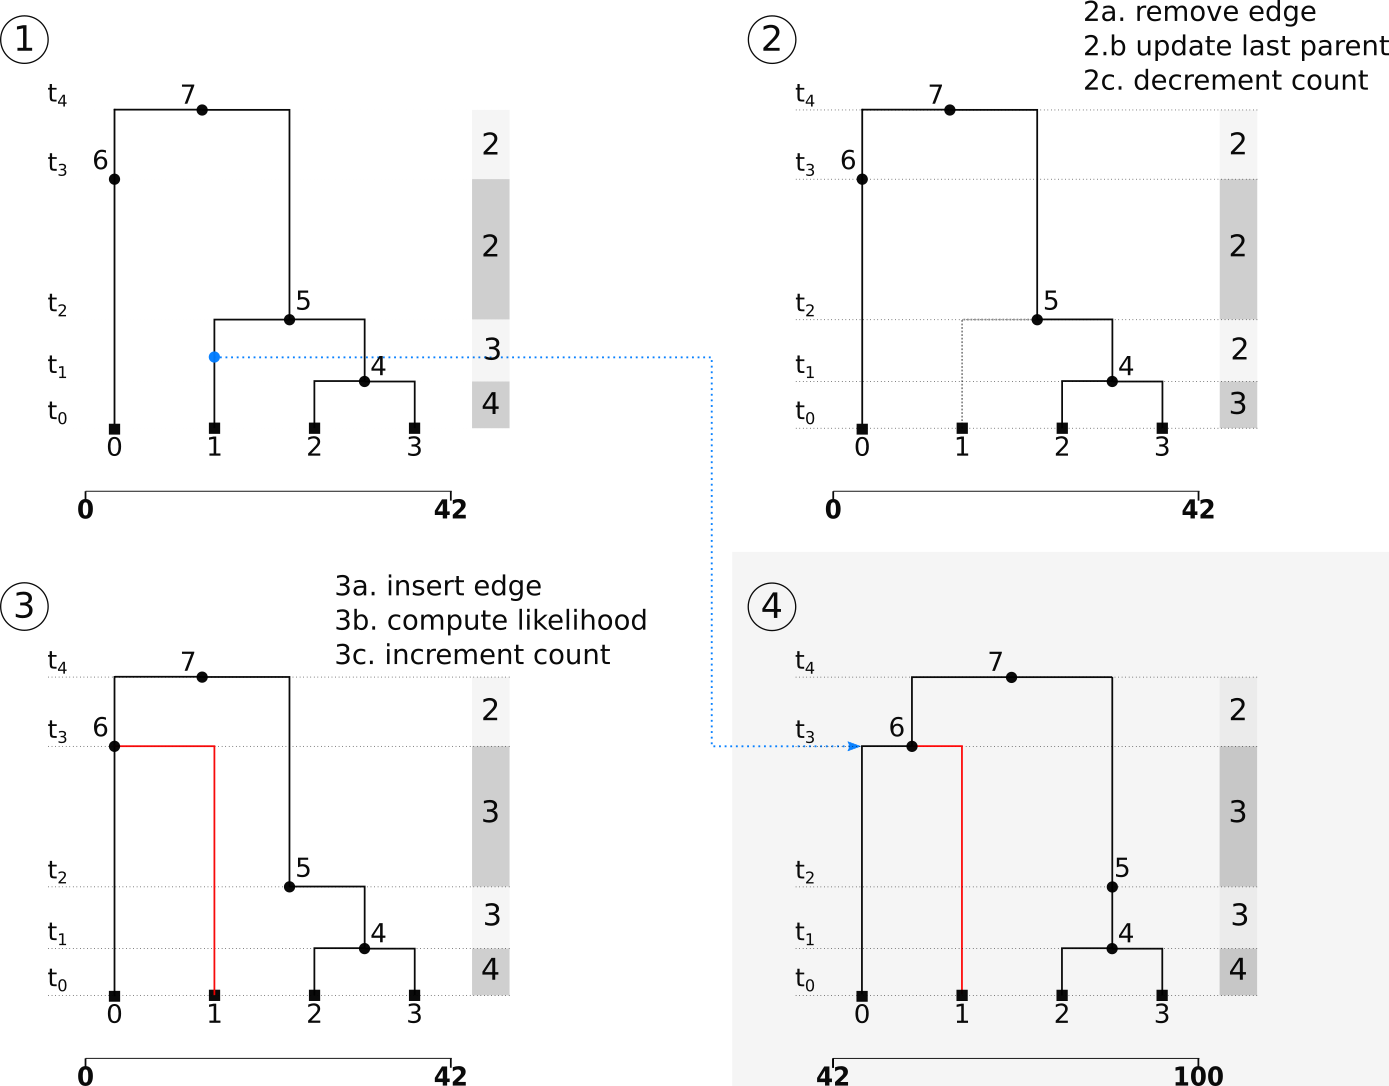
\includegraphics[width=\textwidth]{figures/ts_algo_2rows.png}
\caption{Description of algorithm: Moving along the genome we transition from the first 
local tree (1) to the next (4). For each edge that is removed from the first tree we 
decrement the count in the corresponding internode intervals and update the identity of 
the last parent. Subsequently, for each edge that will be inserted we compute the likelihood 
associated with that edge prior to incrementing the counts.}
\end{figure}


\subsection{Tree sequence format} \label{par:algo}

Although the argument outlined in the previous paragraph is valid for any ARG, here we 
will describe how to (efficiently) extract the information required to associate a
tree sequence encoding of an ARG with a likelihood under the SMC (see fig. \ref{fig:smc-unary}).\\

Formally, we represent a tree sequence using a set of tables \citep{kelleher_efficient_2018}. 
This simple tabular representation of any ARG $\mathcal{G} = (N, E)$, can be 
augmented with additional tables with information on sequence variation
using a site and mutation table. The node table stores information on all 
haplotypes $N$ in the tree sequence. Information about how nodes relate to 
each other along the genome is defined in a tabular encoding of $E$.
Each row in this edge table constitutes a tuple \texttt{(left, right, parent, child)}.
Note that we defined the extent of any edge $\epsilon \in \mathcal{G}$ as the union of 
disjoint intervals. In the tree sequence encoding however, $\epsilon$ will be represented 
by a single entry for each contiguous interval. As remarked before, under the SMC, this 
distinction only matters beyond the root of the genealogy. The distinction between both 
types of edges will therefore not be made in the remainder of the paper.
% Although it does requires us to keep track of some additional information to avoid
% wrongfully assuming a recombination event happened.
% Similarly, the distinction between the lineage associated with an edge, and the edge 
% itself can render things very verbose.
\\

The likelihood computation as described above can be done with a single pass 
of the edge table.
The central problem however is to efficiently maintain the state $I_e(t)$, which counts 
the number of lineages (the lineage associated with) the focal edge $\epsilon$ can coalesce 
with at time $t$. 
The definition of $I_{kl}$ (\ref{def:coal}) is based on the assumption 
that we can impose a strict total order on all (overlapping) lineages based on their 
starting point. The tree sequence encoding provides us with a natural order on all lineages.  
For each local tree with left coordinate $x$, lineages associated with an edge 
starting at $x$ can only coalesce with the subset of lineages associated with one of the
edges that make up that local tree. Each of these edges will either already have 
been present in the previous local tree, or will have the same starting point $x$.
In \texttt{tskit}, the order in which edges are inserted and removed 
while moving from one tree to the next, is determined by the index 
vectors $\textbf{i}$ and $\textbf{o}$ \citep{kelleher_efficient_2016}.
The edge insertion vector $\textbf{i}$ gives the ordering of edges sorted by left 
endpoint, and among edges with the same left endpoint, sorted so that edges closer 
to the root appear later. The edge removal vector $\textbf{o}$ is similar, 
except gives the ordering of edges by right endpoint and with edges closer to the 
root appearing sooner. The variables $\texttt{i}$ and 
$\texttt{o}$ are used to keep track of our position in the edge insertion and edge removal 
indexes as we move along the tree sequence. This order imposes the 
strong ordering on all edges as required by the definition of $I_{kl}$.\\

% edge diff algorithm
The size of the subset of lineages in each internode interval each lineage 
can coalesce with can thus be maintained by keeping track of a single vector $I$ 
that is decremented or incremented as defined by
$\textbf{o}[\texttt{o}]$ and $\textbf{i}[\texttt{i}]$, 
Further keep track of a last-parent array to detect recombination events.
We can thus compute a likelihood for the tree sequence, while visiting each edge only once.

More concretely, prior to inserting an edge, $I$ represents the number of lineages 
the lineage associated with 
that edge can coalesce with. Then insert the edge and update the counts.

To transition from one tree to the next, we first iterate across the indices of all edges 
in $\textbf{o}$ from its current index up to $\texttt{o}$. For each edge in we decrement $I$ 
from index \texttt{edge.child} to \texttt{edge.parent}. We subsequently iterate across the 
edges in $\textbf{i}$ up to index $\texttt{i}$. For each new edge, we first compute the likelihood 
associated with that edge and then 
increment $I$ from \texttt{edge.child} to \texttt{edge.parent}.\\

% ADD IN RESULTS
Figure \ref{sup:fig:vs-hudson} shows the correlation between the likelihood under the hudson 
for an ARG with detailed recombination information simulated and computed using 
\texttt{msprime} \citep{baumdicker_efficient_2021}. Show impact of unary nodes on $r^2$.
Simulated mutation data under the SMC and passed this to ARGweaver.
Scatterplot of coalescent prior as returned by ARGweaver \citep{rasmussen_genome-wide_2014} 
for a 100 samples from the posterior against the likelihood as described here fore these 
sampled ARGs \ref{sup:fig:vs-argweaver}  

Implementation of the algorithm is available on https://github.com/GertjanBisschop/runsmc.

\subsection{Flexibility / general class of ARGs}

% slicing of the ARG
By explicitly associating a single likelihood with each edge, we can compute a likelihood 
under the SMC for any valid tree sequence. The \texttt{tskit} library provides a whole range  
of subsetting operations on tree sequences allowing us to slice the ARG in time and/or space, 
as well as reduce the number of tracked samples. 
Any such subset of the tree sequence is itself a valid tree sequence 
that can again be used to compute a likelihood with.

Our approach therefore strenghtens the inherent ability of ARGs to provide us with temporal 
resolution on the inferred genealogical history of a sample. 
We can further readily incorporate changes in $N_e$ and $r$, 
both in time as well as along the genome.

% Algorithm is suitable for a general class of ARGs each with their own specific features.
% What happens in the case of ARGs that do not meet our assumptions: absent unary nodes, polytomies, ...
The above algorithm treats each edge independently which implies we can deal with polytomies.
Furthermore, although we rely heavily on unary nodes to provide us with the necessary 
information on recombination events, our algorithm can also accomodate for 
those inferred ARGs that lack unary nodes (e.g.\ \relate, and see figure in supplements).
However, in case of (sub)tree height changes along the ARG, the algorithm would infer 
two recombination events along the lineages associated 
with both edges switching parent nodes. This can be mitigated by limiting the number of 
'inferrable' recombination events per coalescence event to 1 (see supplementary figure). 


\section{Discussion}
% summary: what did we do here
Here, we have introduced a scalable algorithm to compute likelihoods 
under the SMC for a general class of ARGs. 



Impact both on ways of doing ARG inference itself and quantifying the uncertainty associated 
with that as well as performing statistical inference of past demography.

* statistical inference *
This is an important step towards bridging the gap between the tremendous 
recent advances in ARG inference and the current state of the art statistical inference of 
past demography (but see ). 
% some/many of these approaches only use the information present in marginal trees.
The provided theory and associated algorithm will function as a building block of a 
demography-aware genealogy sampler. Current approach couple of major advantages:
* any type of inferred ARG as a starting point. Potentially implying a massive reduction in 
MCMC runtime by reducing the necessary burnin period.
* by integrating out the exact time to the recombination event we further restrict the size 
of ARG space that needs to be explored.
* exploit the efficiencies of the tree sequence data structure (see \citep{Mahmoudi_bayesian_2022})
* we can readily incorporate $N_e$-changes as well as multiple populations and migration.


* ARG inference *
Combining ARG inference methods: tsinfer for first few generations (large sample sizes), where 
the initial phase is biased relative to the Wright-Fisher model when the sample size is large 
\citep{bhaskar_distortion_2014}, or when the considered events are very recent \citep{wakeley_gene_2012}
% tsinfer not model-based, minimal assumptions, heuristic, scalable



quantify uncertainty
* polytomies represent uncertainty:
*  systematicallty break them by sampling from the coalescent rather then randomly
* associate uncertainty as metadata to parent node representing uncertainty in the
* interval spanned by the polytomy
* can something similar be done for stacked recombinations?




\bibliographystyle{plainnat}
\bibliography{paper.bib, temp.bib}

\pagebreak 

\supplementarysection
\section*{Supplementary Information}


\begin{figure}[!ht]
\centering
\includegraphics[width=0.5\textwidth]{example-image-a}
\caption{Compare likelihoods inferred ARGs ARGweaver}
 \label{sup:fig:vs-argweaver}
\end{figure}


\begin{figure}[!ht]
\centering
\includegraphics[width=0.5\textwidth]{example-image-a}
\caption{Compare likelihoods Hudson and SMC}
\label{sup:fig:vs-hudson}
\end{figure}

\end{document}
